% ##CHRIS 2026-09-22: converted to IEEEtran (journal, two columns). Level 3 box added, marked
% "v4 pending". Every claim carries its % TODO-source line.
\documentclass[journal]{IEEEtran}
\usepackage{amsmath,amssymb,booktabs,graphicx,microtype,enumitem}
\usepackage[dvipsnames]{xcolor}
\usepackage[colorlinks=true,linkcolor=NavyBlue,urlcolor=NavyBlue]{hyperref}
\newcommand{\kT}{k_{\mathrm B}T}
\newcommand{\avg}[1]{\left\langle #1 \right\rangle}
\newcommand{\dd}{\mathrm{d}}
\graphicspath{{../experiments/final/}}

\begin{document}

\title{Where injected work goes in a hard-disk box:\\
a proof ladder for an energy-transfer experiment}

\author{Christoph~Haring and Susanne~Still%
\thanks{The authors are with the Department of Information and Computer Sciences,
University of Hawai\`i at M\=anoa, Honolulu, HI 96822 USA
(e-mail: charing@hawaii.edu; sstill@hawaii.edu).}}

\maketitle


\begin{abstract}
A piston compresses a hard-disk gas in a closed box. We ask what fraction of the injected work can
still be captured as ordered energy, and we refuse to answer until each simpler statement below it is
closed: the ledger, the quasi-static baseline, the finite-rate excess, the spring, the divider, the
chain. Levels 0--2 are closed here.
% TODO-source: Level status from 260913_tests_STATUS.md, 2026-09-16 .. 2026-09-19
The headline of Level 2 is that a closed compartment has \emph{no} linear friction: the force
autocorrelation of a held piston integrates to zero at the sound traversal time, and the finite-rate
cost is second order, $\avg W - W_{\mathrm{qs}} = A u^2$, of which roughly half is energy the
protocol itself launches.
\end{abstract}
\begin{IEEEkeywords}
hard-disk fluid, energy transfer, event-driven molecular dynamics, dissipation, adiabatic piston
\end{IEEEkeywords}


\section{The box and the ladder}
Geometry A: two compartments of $N_s = 50$ disks either side of an immovable divider, a piston on the
right. $\kT = m = \sigma = 1$, $H = 10$, compartment $38.75\,\sigma$, gas compression
$\Delta x = 3.93\,\sigma$.
% TODO-source: geometry established in section 1 of 260919_paper2_ramp_linewidth_fast_REPORT.md
\begin{figure*}[t]\centering

\includegraphics[width=0.48\textwidth]{260920_master_geomA_paper.png}\hfill

\includegraphics[width=0.48\textwidth]{260920_master_geomB_paper.png}\\[3pt]
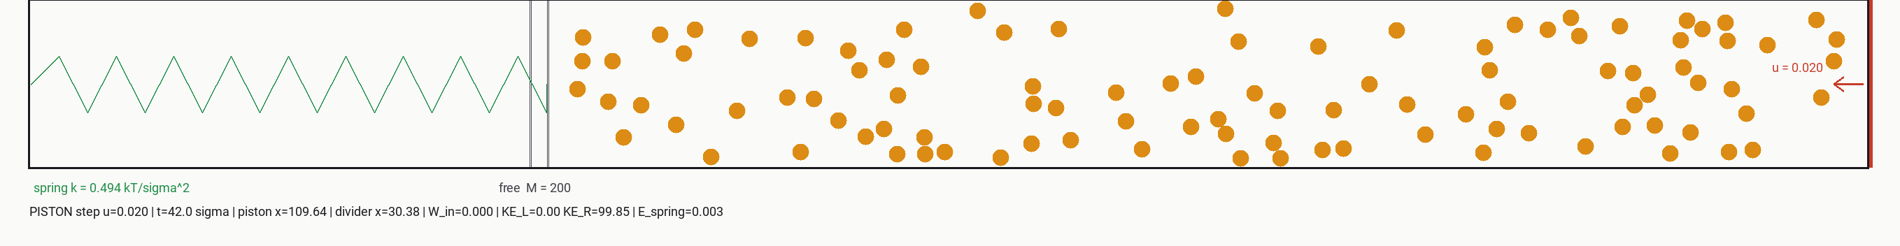
\includegraphics[width=0.48\textwidth]{260920_master_geomC_paper.png}\hfill

\includegraphics[width=0.48\textwidth]{260920_master_geomD_paper.png}
\caption{The master box, one apparatus with elements switched on. A (top left) both walls held, as
Levels 0--2 were measured; B (top right) divider free; C (bottom left) divider removed, one gas
driving the spring-loaded wall; D (bottom right) both free. Held walls are drawn solid and labelled
by mass, free walls hollow; the spring is grey when held and green when live.}
\label{fig:geoms}
\end{figure*}

\section{Level 0 --- the ledger closes}
$R_E = W - [\Delta KE_{\mathrm{gas}} + \Delta KE_{\mathrm{walls}} + \Delta E_{\mathrm{spring}} + Q]$
and the matching momentum residual, from the per-event impulse log.
% TODO-source: 260917_paper2_level0_level1_REPORT.md
\textbf{Measured:} $|R_E|/W \le 8\times10^{-12}$, $|R_p|/\sum|\Delta p| \le 1\times10^{-13}$ over all
75 pilot trajectories. \textbf{Passed.}

\section{Level 1 --- the quasi-static baseline}
$W_{\mathrm{qs}} = N_s\kT(T_f/T_i - 1)$ with $\ln(T_f/T_i) = \int Z\,\dd\ln\eta$ along the path, $Z$
measured in the finite box rather than taken from the bulk EOS.
% TODO-source: paper2_geometry_fix_20260918.py, 5 path points, 100 holds each
\textbf{Measured:} $W_{\mathrm{qs}}^{\mathrm{finite}} = 7.4685 \pm 0.0131\,\kT$; extrapolating the
measured work to $u \to 0$ with the (quadratic) form gives $W(0) - W_{\mathrm{qs}} = +0.0043 \pm
0.0158\,\kT$, $0.3\sigma$. \textbf{Passed}, and on the physical side.

\section{Level 2 --- the finite-rate excess}
\subsection{Slow end}
\begin{equation}
\zeta(\lambda) = \beta\int_0^\infty \avg{\delta F(0)\,\delta F(t)}\,\dd t , \qquad
W_{\mathrm{diss}} \simeq \zeta\,u\,\Delta x .
\end{equation}
% TODO-source: 260917_paper2_level2_REPORT.md sections 2-4 and appendix A of the 260919 report
\textbf{Measured:} the integral is not Markovian. It falls from $2.55$ at zero lag --- the Enskog
collisional friction --- and is cancelled by the returning sound wave at $L/c_s = 19.8\,\sigma$,
confirmed at the compressed end of the path where the crossing moves to $18.0\,\sigma$ against a
predicted $15.9$. Its zero-frequency limit is the hydrodynamic viscous friction
$\zeta_{\mathrm{hyd}} = L_y\Gamma/X_p = 0.081 \pm 0.010$, which predicts a linear term of
$0.32 \pm 0.04\,u$ --- below the resolution of 760 trajectories, and consistent with the measured
slope $-0.50 \pm 0.67$ for $u \le 0.05$. $\Gamma$ is taken from Paper 1's divider linewidth, not
assumed.

\textbf{What is there instead} is quadratic: $A_{\mathrm{step}} = 25.9 \pm 4.3$ against
$A_{\mathrm{ramp}} = 11.3 \pm 2.5$ when the piston is ramped over $2L/c_s$ instead of stepped
($3.0\sigma$ apart). Roughly $14$ of the $25$ is energy the step protocol launches; what a gentle
push leaves is consistent with the steady-flow value $N_s m/6 = 8.3$.

\subsection{Fast end}
$\avg W \simeq 2 N_s m (\Delta x/L) u^2$, no free parameter.
% TODO-source: appendix C3 of the 260919 report
\textbf{Measured:} $0.986$ of prediction at $u = 10$, $\Delta x = 7.08\,\sigma$. The apparent
$8\,\%$ excess at short travel is the contact layer: the strip a face can strike (width $\Delta x$
starting at face $-\,r$) holds $1.13\times$ the uniform-density count at $\Delta x = 0.75\,\sigma$.
Using the measured count the ratio becomes $0.96$--$1.03$ with no trend.

\begin{figure}[htbp]\centering
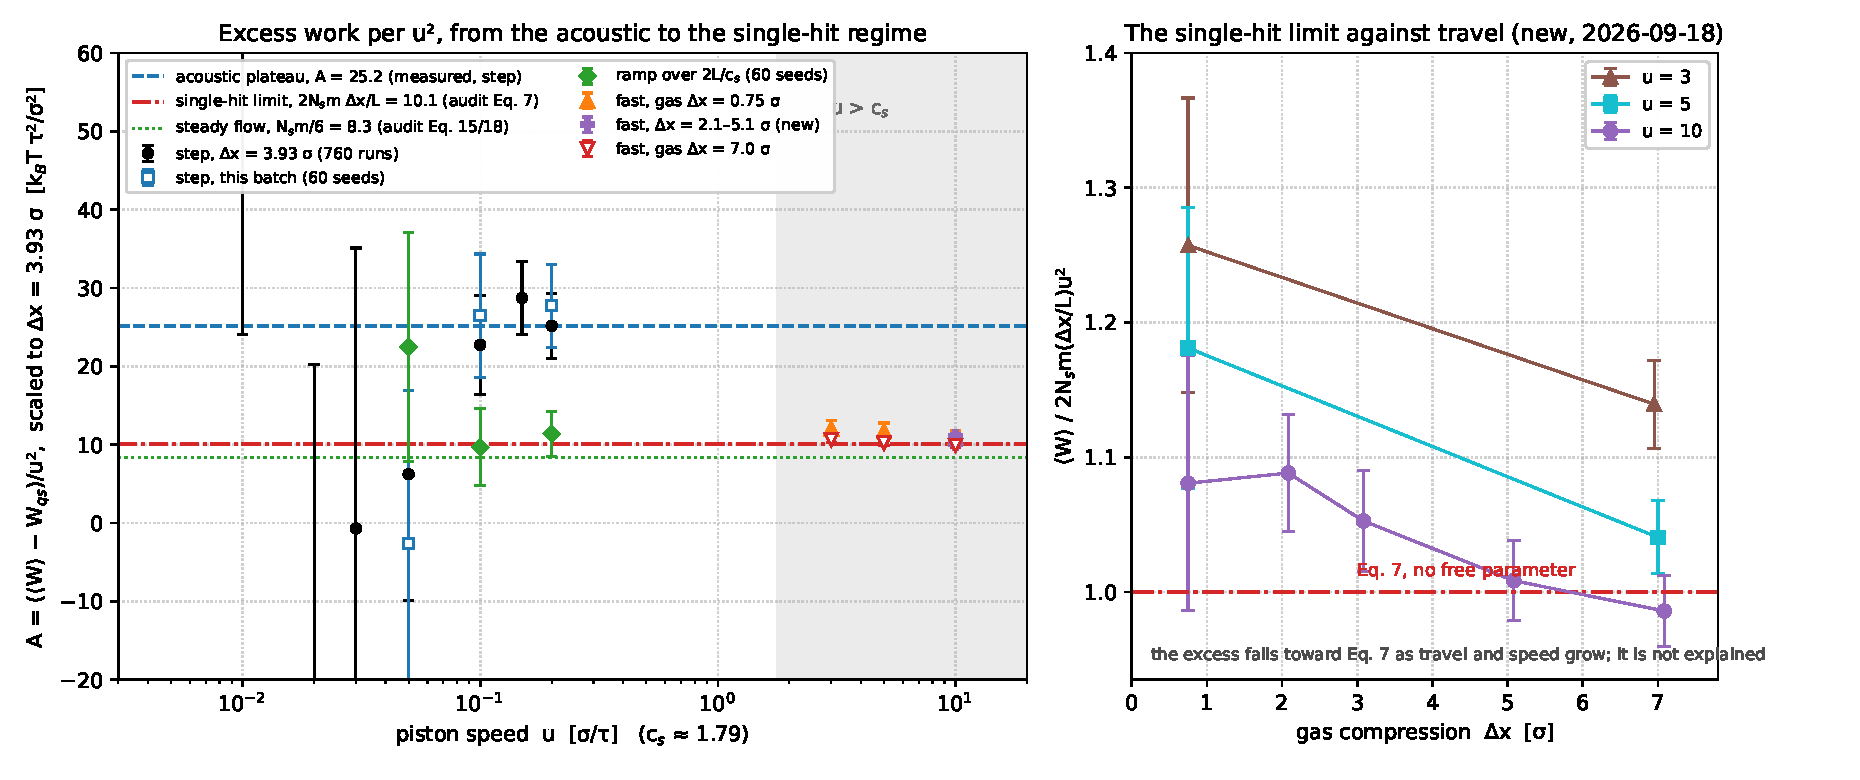
\includegraphics[width=\linewidth]{260918_level2_A_of_u.pdf}
\caption{$A(u) = (\avg W - W_{\mathrm{qs}})/u^2$ from the acoustic to the single-hit regime, every
point scaled to a common travel, with the travel scan at right.}
\end{figure}

\section{Level 3 --- can a spring capture it?}\label{sec:l3}
\emph{Closed on the observable (2026-09-25).} Geometry C: one gas of 100 disks drives a spring-loaded wall through a
10\,\% compression ($\Delta x = 7.96\,\sigma$, $\eta$ $0.100 \to 0.111$).
% TODO-source: 260921_paper2_level3_REPORT_v3.md, 260922_paper2_level3_REPORT_v4.md

\textbf{The apparatus is a pre-loaded spring.} It holds the standing gas force
$F = N\kT Z/L$, so the wall sits $d = F/k$ from the anchor and
$\Delta E = F s + \tfrac12 k s^2$ is \emph{first} order in the wall displacement --- the $Fs$ term
is work lifting a weight. Limits: $k \to 0$ is a pushrod ($\epsilon \to 1$ trivially, nothing taken
from the gas), $k \to \infty$ a rigid wall ($\epsilon \to 0$).

\textbf{The gas spring is adiabatic, and it is Paper 1's $c_s$.} With $U = N\kT$ in 2D,
$\dd U = -P\,\dd V$ gives $\dd\ln T/\dd\ln L = -Z$ and
$k_{\mathrm{gas}} = (N\kT/L^2)\,c_s^2$ --- which is also the heavy-divider limit of
Rom\'an's $\cot K = \alpha K$, so the two papers share one line of physics. It is $2.01\times$ the
isothermal stiffness here, and the adiabat reproduces Level 1's measured $T_f/T_i = 1.149$ to
$0.5\,\%$.

\textbf{Status: closed on the observable.} The ledger closes (median $4.6\times10^{-10}$,
593/600 below $10^{-8}$). The observable is the wall's settled displacement, pooled over five cells
with validated windows, $\bar s = 0.8705 \pm 0.0049\,\sigma$. The gas input is the box's own
measured pressure: in equilibrium the force a hard wall feels is the pressure of the box
($P = k_BT\rho_{\mathrm{contact}}$, uniform normal pressure), and it is what the spring wall feels,
so $Z_{\mathrm{box}}(\eta) = FL/(Nk_BT)$ is measured directly from the momentum delivered to a held
wall. With it the parameter-free model $M\ddot s = F(L - x_p + s) - F(L) - k s$ predicts the settled
displacement to $-1.3 \pm 0.6\,\%$ ($2.2\sigma$); with the bulk equation of state, $+3.6\,\%$.

The box is $2.5\,\%$ over-pressured relative to Kolafa--Rottner and $1.0\,\%$ over-stiff in $c_s$
(Paper~1). Through $c_s^2 = Z + \eta Z' + Z^2$ the first would imply $+1.9\,\%$ in $c_s$, so the two
finite-size numbers do not agree, at roughly $3\sigma$; both are reported. The transient excess
reported earlier was a peak statistic, reproduced by a no-push control with no gas driving at all.

\section{Level 4 --- transmission through a free divider}
\emph{Not started.} Fast pressure channel against slow heat channel;
$\mathcal{T}(t) = \Delta KE_{\mathrm{gas\,2}}(t)/W_{\mathrm{in}}$, with
$\mathcal{T}_{\mathrm{slow}} \to 1/2$ for symmetric gases.

\section{Level 5 --- the chain}
\emph{Not started.} $\epsilon = E_{\mathrm{spring,max}}/W_{\mathrm{in}}$ against piston speed,
divider mass and the number of walls; the prediction is the \emph{ordering}, geometric intermediate
masses beating badly matched ones.


\section{Level 6 --- information}
\emph{Not started, and gated on a canonical seeder.} $\beta\avg{W_{\mathrm{diss}}} \ge
I_{\mathrm{mem}} - I_{\mathrm{pred}}$. Note that the Jarzynski benchmark must be the finite-box
$\Delta F$, exactly as Level 1 needed the finite-box $W_{\mathrm{qs}}$.

\section*{Reproducibility}
Raw trajectories are not in the repository; each cell carries \texttt{summary.csv} and
\texttt{00\_COMMAND.md}, and Level 2 an 85\,kB \texttt{stop\_digest.csv} from which the entire
analysis reproduces. Batch scripts are in \texttt{../experiments/run\_scripts/}.

\end{document}
